\documentclass[a4paper,11pt]{article}
\usepackage[a4paper,margin=0.3cm,rmargin=1cm]{geometry}
\usepackage{graphicx}
\usepackage{parskip}
\usepackage{enumitem}
\usepackage{csquotes}
\usepackage{hyperref}
\usepackage{xcolor}
\usepackage{avant} % for font
\usepackage{titlesec}
\usepackage[many]{tcolorbox}
\tcbuselibrary{skins,breakable} % Load necessary libraries


\renewcommand{\familydefault}{\sfdefault}

\titlespacing*{\section}{0pt}{8pt}{4pt}
\newcommand{\subsectionskip}[0]{\vspace{0.125cm}}

% rm left indent
\setlength{\parindent}{0pt}

% compact enumerations
\setlist{noitemsep,topsep=0pt,leftmargin=*}
% \setitemize{noitemsep,topsep=0pt,parsep=0pt,partopsep=0pt}

% include path for images
\graphicspath{ {./images/} }

\newcommand{\col}[2]{\textcolor[HTML]{#1}{#2}}
\newcommand{\badge}[1]{\tcbox[on line,size=small,nobeforeafter,fontupper={\strut},bottom=-0.75mm]{\textbf{#1}}}
\input{variables.tex} % include GitHub URL and commit string

\begin{document}

% banner on left side
\noindent
\begin{minipage}[t]{0.3106\textwidth}
    \clearpage  % fix for page break before content
    \vspace{-0.45cm}
    
\includegraphics[width=\textwidth]{triangles.pdf}
    \begin{center}
    \tiny \col{316dbc}{\textbf{made with \href{https://github.com/louisradtke/cv-banner}{github.com/louisradtke/cv-banner}}}
    \end{center}

    % profile picture
    \vspace{-26.92cm}
    \begin{center}
        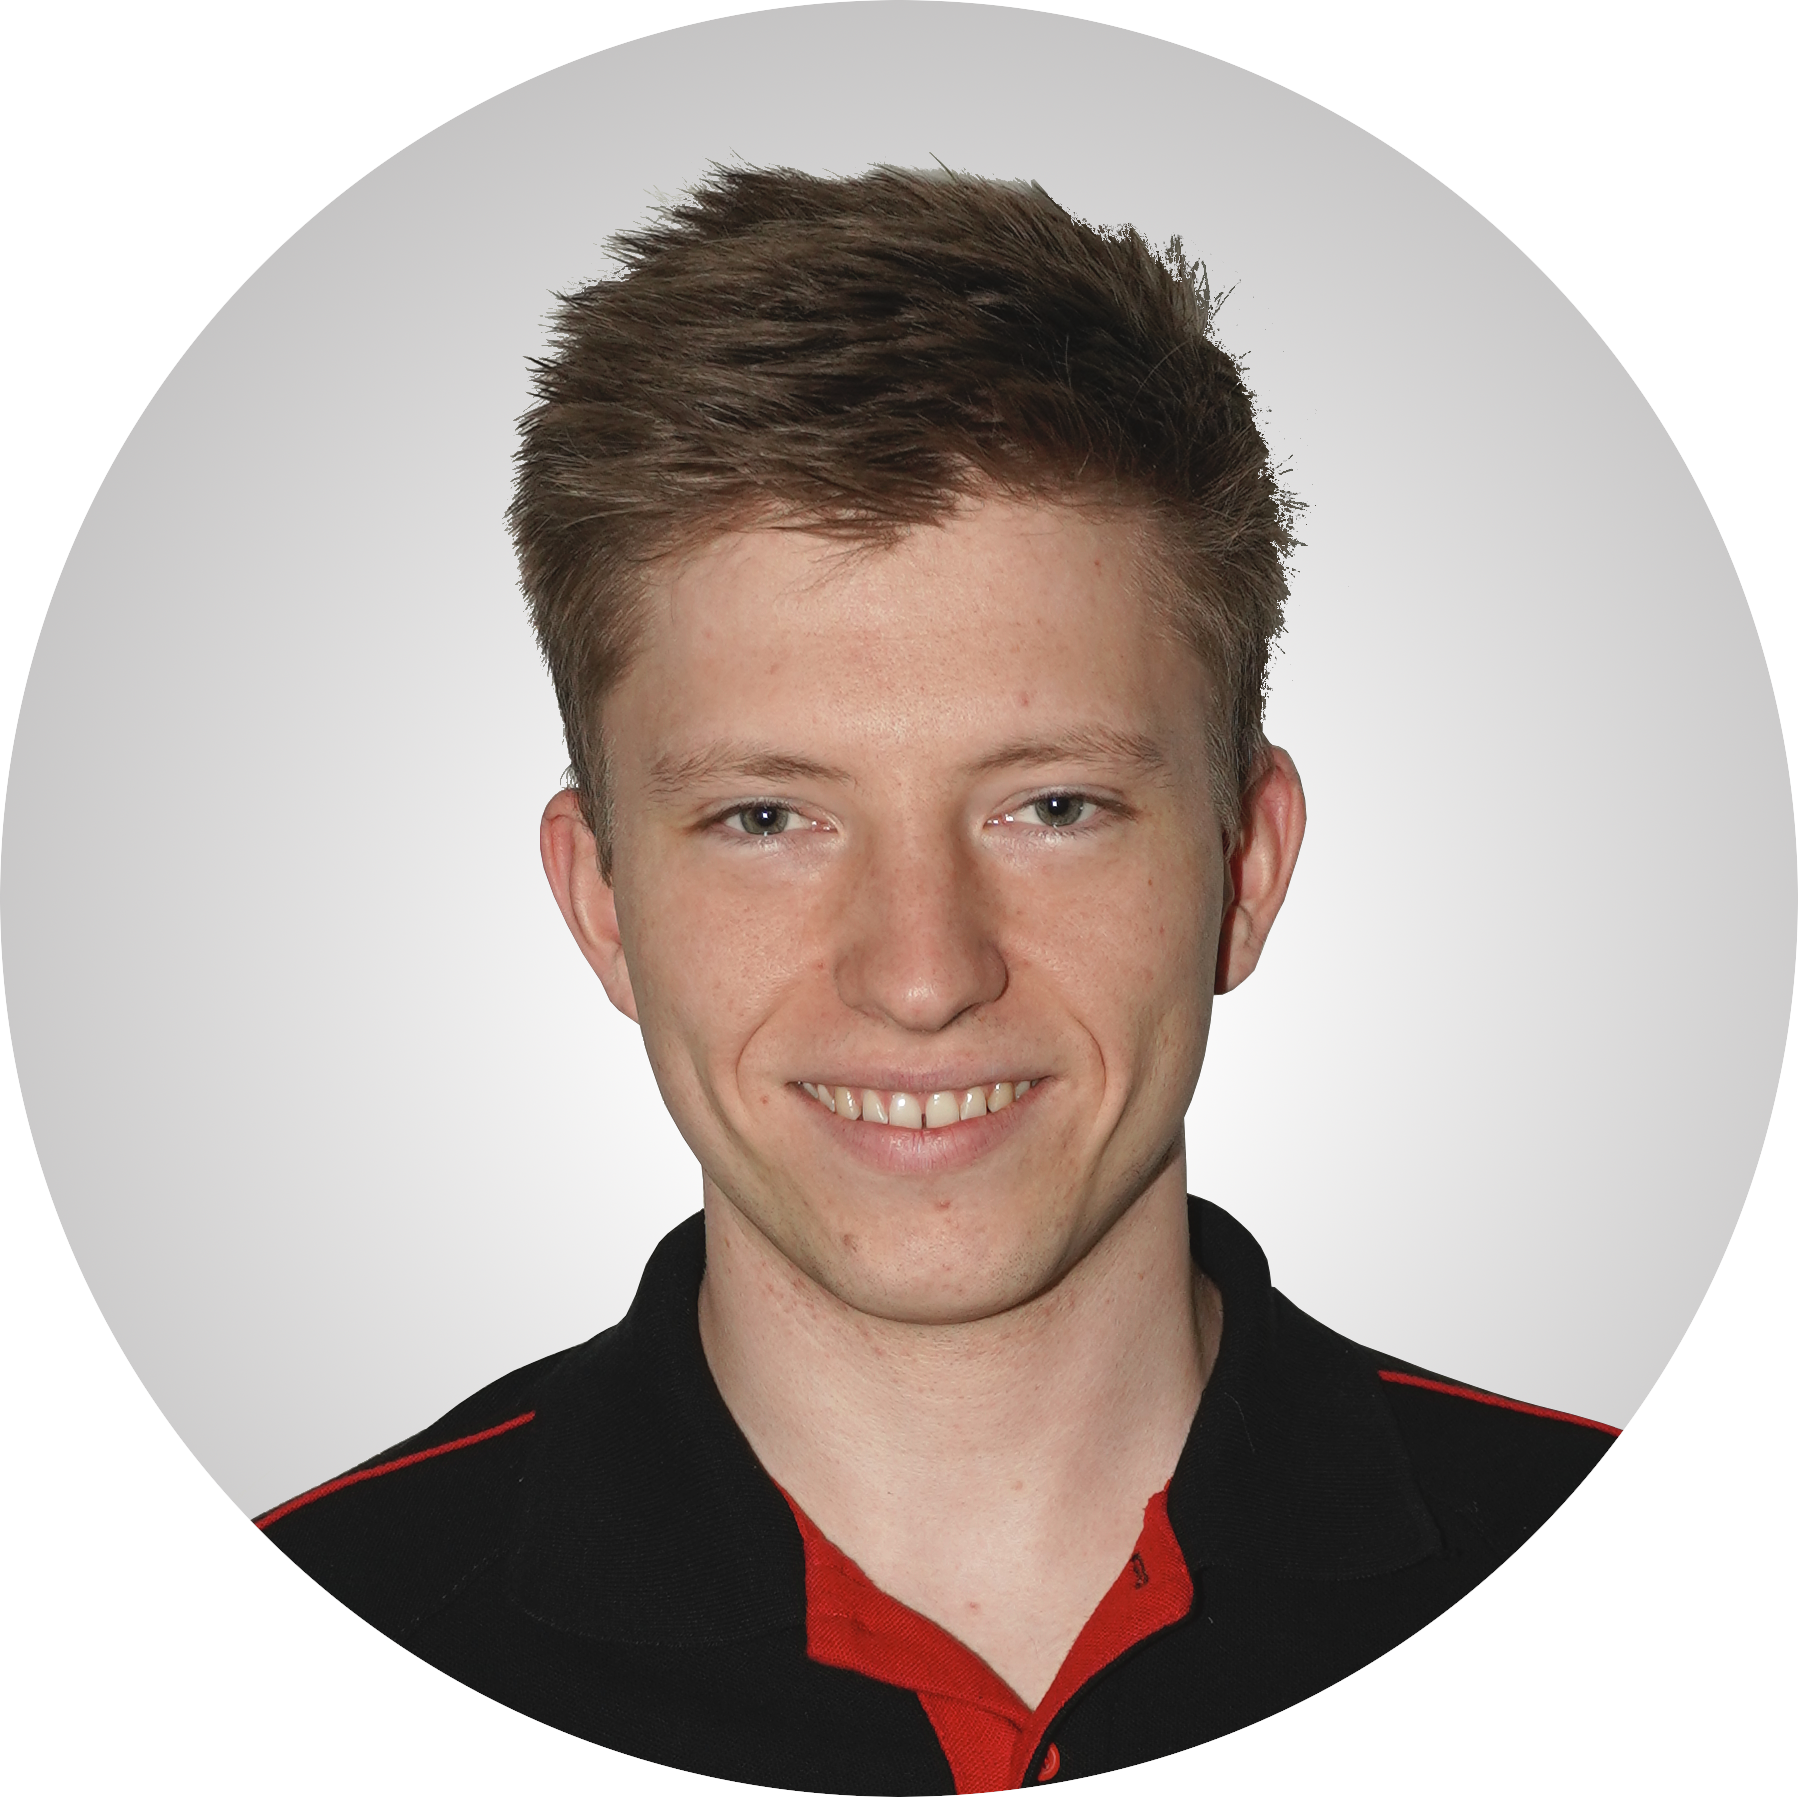
\includegraphics[width=4.5cm,clip]{profile.png}
    \end{center}

    \vspace{1.02cm}
    \begin{center}
    \begin{minipage}[t][5cm][t]{0.72\textwidth}
        \centering
        engineering software \& robotic systems\\
        \vspace{0.125cm}
        \small
        \badge{.NET} \badge{Python} \badge{C++}
        \badge{Linux} \badge{Management}

        % software engineer,\\
        % robotics engineer,\\
    \end{minipage}
    \end{center}

    \vspace{13.25cm}
    \begin{center}
    \begin{minipage}{0.72\textwidth}
        \centering
        % \textsc{\textbf{Louis Radtke}}\\
        % \huge\col{c6997c}{\textbf{Louis Radtke}}\\
        \large\textbf{Louis Radtke, B.Sc.}\\
        \vspace{0.12cm}
        \scriptsize born January 1999, Hagen, DE\\
        louisradtke.dev@gmail.com\\
        \url{https://louisradtke.dev}
        % \normalsize software engineer\\
        % robotics engineer
    \end{minipage}
    \end{center}

    % text block 1:
    % Louis Radtke, B.Sc.
    % sth. w/ software engineer, robotics engineer, workflow optimizer, team player

    % footer for flow: made with github.com/louisradtke-cv-flow
\end{minipage}
\hfill
\begin{minipage}[t]{0.65\textwidth}
    \vspace{0cm} % fix for misalignment with top margin
    \begin{center}
        \title*{\Huge \textbf{Louis Radtke}}\\
        % \textsc{\textbf{Curriculum Vitae}}
        % \title*{\Huge \col{c67e43}{\textsc{\textbf{Curriculum Vitae}}}}
    \end{center}

    \vspace{0.125cm}

    {
        \small A Masters CS student with 5 years of project experience in software development, including the deployment of software in demanding real-world applications. Former captain/CEO of a Formula Student team and founder of their automated driving section. Dedication for technology, software architecture and workflow optimization.
    }

    % to do: summary about professional profile. carer goals? highlight of key achievements. aspiring software architect. focus developer and user experience. optimize workflows.

    \vspace{0.25cm}
    \hrule

    \section*{\col{ac7448}{Experience}}
    \col{b27c52}{\textbf{Research Assistant \hfill 2024 -- Today}}\\
    AQUA Research Group, TU Dortmund, DE
    \begin{itemize}
        \small
        \item Preparation of the research data infrastructure.
        \item Support in procurement of an FSD testing vehicle.
    \end{itemize}

    \subsectionskip

    \col{b3805b}{\textbf{Software Engineer \hfill 2018 -- Today}} \\
    SimPlan Integrations GmbH, Witten, DE
    \begin{itemize}
        \small
        \item Unsupervised implementation of customer and internal projects.
        \item Introduction of GitLab for managing code, tasks and as QA tool.
    \end{itemize}

    \subsectionskip

    \col{b38668}{\textbf{Team Captain / CEO \hfill 2023}} \\
    GET racing, Formula Student Team of TU Dortmund, DE
    \begin{itemize}
        \small
        \item Coordination of the production phase of the FS223 vehicle.
        \item Integration of autonomous driving software with electro-mech. systems.
        \item Logistical planning of the competitions.
    \end{itemize}

    \subsectionskip

    \textbf{\col{a68573}{Autonomous System Lead \hfill 2019 -- 2023}} \\
    GET racing, Formula Student Team of TU Dortmund, DE
    \begin{itemize}
        \small
        \item Initial assembly of the autonomous system department.
        \item Acquisition of partners in industry and at university.
        \item Conception and implementation of the autonomous system software.
        \item Commissioning and development of automated simulation infrastructure.
        \item Introduction of new PM tool (JetBrains YouTrack) to entire team.
    \end{itemize}

    \section*{\col{908587}{Education}}
    \col{91878a}{\textbf{M.Sc. in Computer Science \hfill 2022 -- Today}} \\
    TU Dortmund, DE
    \begin{itemize}
        \small
        \item Seminar: AI in Software Engineering -- built RAG pipeline using LLMs
        \item Project group: \enquote{Continuous and Compositional Validation}
        \item Research project: building a research data management system
        \item Courses on software engineering, computer graphics, pattern recognition, real time operating systems and deep \& reinforcement learning (AI)
    \end{itemize}

    \subsectionskip

    \col{81879c}{\textbf{B.Sc. in Applied Computer Science \hfill 2017 -- 2022}} \\
    TU Dortmund, DE
    \begin{itemize}
        \small
        \item Minor subject: Robotics (controls theory and electronics)
        \item Thesis: A method for localizing mobile robots using multiple sensors
    \end{itemize}

    \subsectionskip

    \col{81879c}{\textbf{Abitur \hfill 2009 -- 2017}} \\
    Gymnasium Hohenlimburg, Hagen, DE

    \vspace{-0.5cm} % dirty fix for space above minipage

    \begin{minipage}[t]{0.625\textwidth}
        \col{7690bb}{\section*{Skills \& Certificates}}
        \begin{itemize}
            \small
            \item Programming \& Ecosystems:\\
            .NET (\textbf{++++}), Python (\textbf{++++}), C++ (\textbf{+++}),\\
            C (\textbf{++}), JS/TS/WebTech (\textbf{++}), Java/Kotlin (\textbf{++})

            \item Systems \& Administration:\\
            Linux (\textbf{++++}, daily use), Bash (\textbf{+++}) \\
            Docker (\textbf{++++}), GitLab CI (\textbf{++++})

            \item Circuit and 3D design, manufacturing CFC.

            \item Windows and MS office suite (\textbf{+++}).

            \item Management of diverse teams of software, electrical and mechanical engineers, as well as the business operations team.

            \item Project Management Tools:\\
            GitLab (\textbf{++++}), JetBrains YouTrack (\textbf{+++})

            \item Licenses: A, B, SBF Inland \& Sea
        \end{itemize}
    \end{minipage}
    \hfill
    \begin{minipage}[t]{0.325\textwidth}
        \col{ffffff}{.} % dirty fix for v misalignment of headings
        \section*{\col{7690bb}{Languages}}
        \begin{itemize}
            \small
            \item German -- Native
            \item English -- Fluent
            \item French -- Basic
        \end{itemize}

        \section*{\col{6187bd}{Freetime}}
        \begin{itemize}
            \small
            \item Jogging \& bouldering
            \item Sailing
            \item Private projects with electronics and 3D design
            \item 2014: Volunteer in a retirement home
        \end{itemize}
    \end{minipage}

\end{minipage}

\vfill
\hfill
\vspace{0.17cm}
\begin{minipage}[t]{0.65\textwidth}
    \hrule
    \vspace{0.125cm}

    \small build \href{\giturl}{\texttt{\gitcommit}} \hfill \today
\end{minipage}

\end{document}
